% !TeX spellcheck = es_ANY
% Chapter 1

%\chapter{Chapter Title Here} % Main chapter title
%
%\label{Chapter1} % For referencing the chapter elsewhere, use \ref{Chapter1} 

%----------------------------------------------------------------------------------------

% Define some commands to keep the formatting separated from the content 
%\newcommand{\keyword}[1]{\textit{#1}}
%\newcommand{\tabhead}[1]{\textbf{#1}}
%\newcommand{\code}[1]{\texttt{#1}}
%\newcommand{\file}[1]{\texttt{\bfseries#1}}
%\newcommand{\option}[1]{\texttt{\itshape#1}}

%----------------------------------------------------------------------------------------

\chapter{Imágenes de soporte}\label{anx: imagenes}
	\begin{figure}[!h]
		\centering
		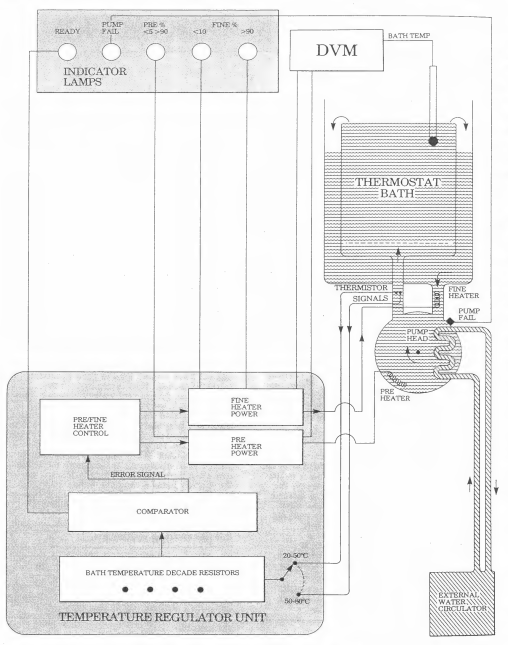
\includegraphics[height =0.65\textheight]{Figures/controlTemperatura}
		\caption{Control t\'ermico del calor\'imetro. Modificado de \cite{Suurkuusk}.}
		\label{fig: controlTermico}
	\end{figure}

	\begin{figure}[!h]
		\centering
		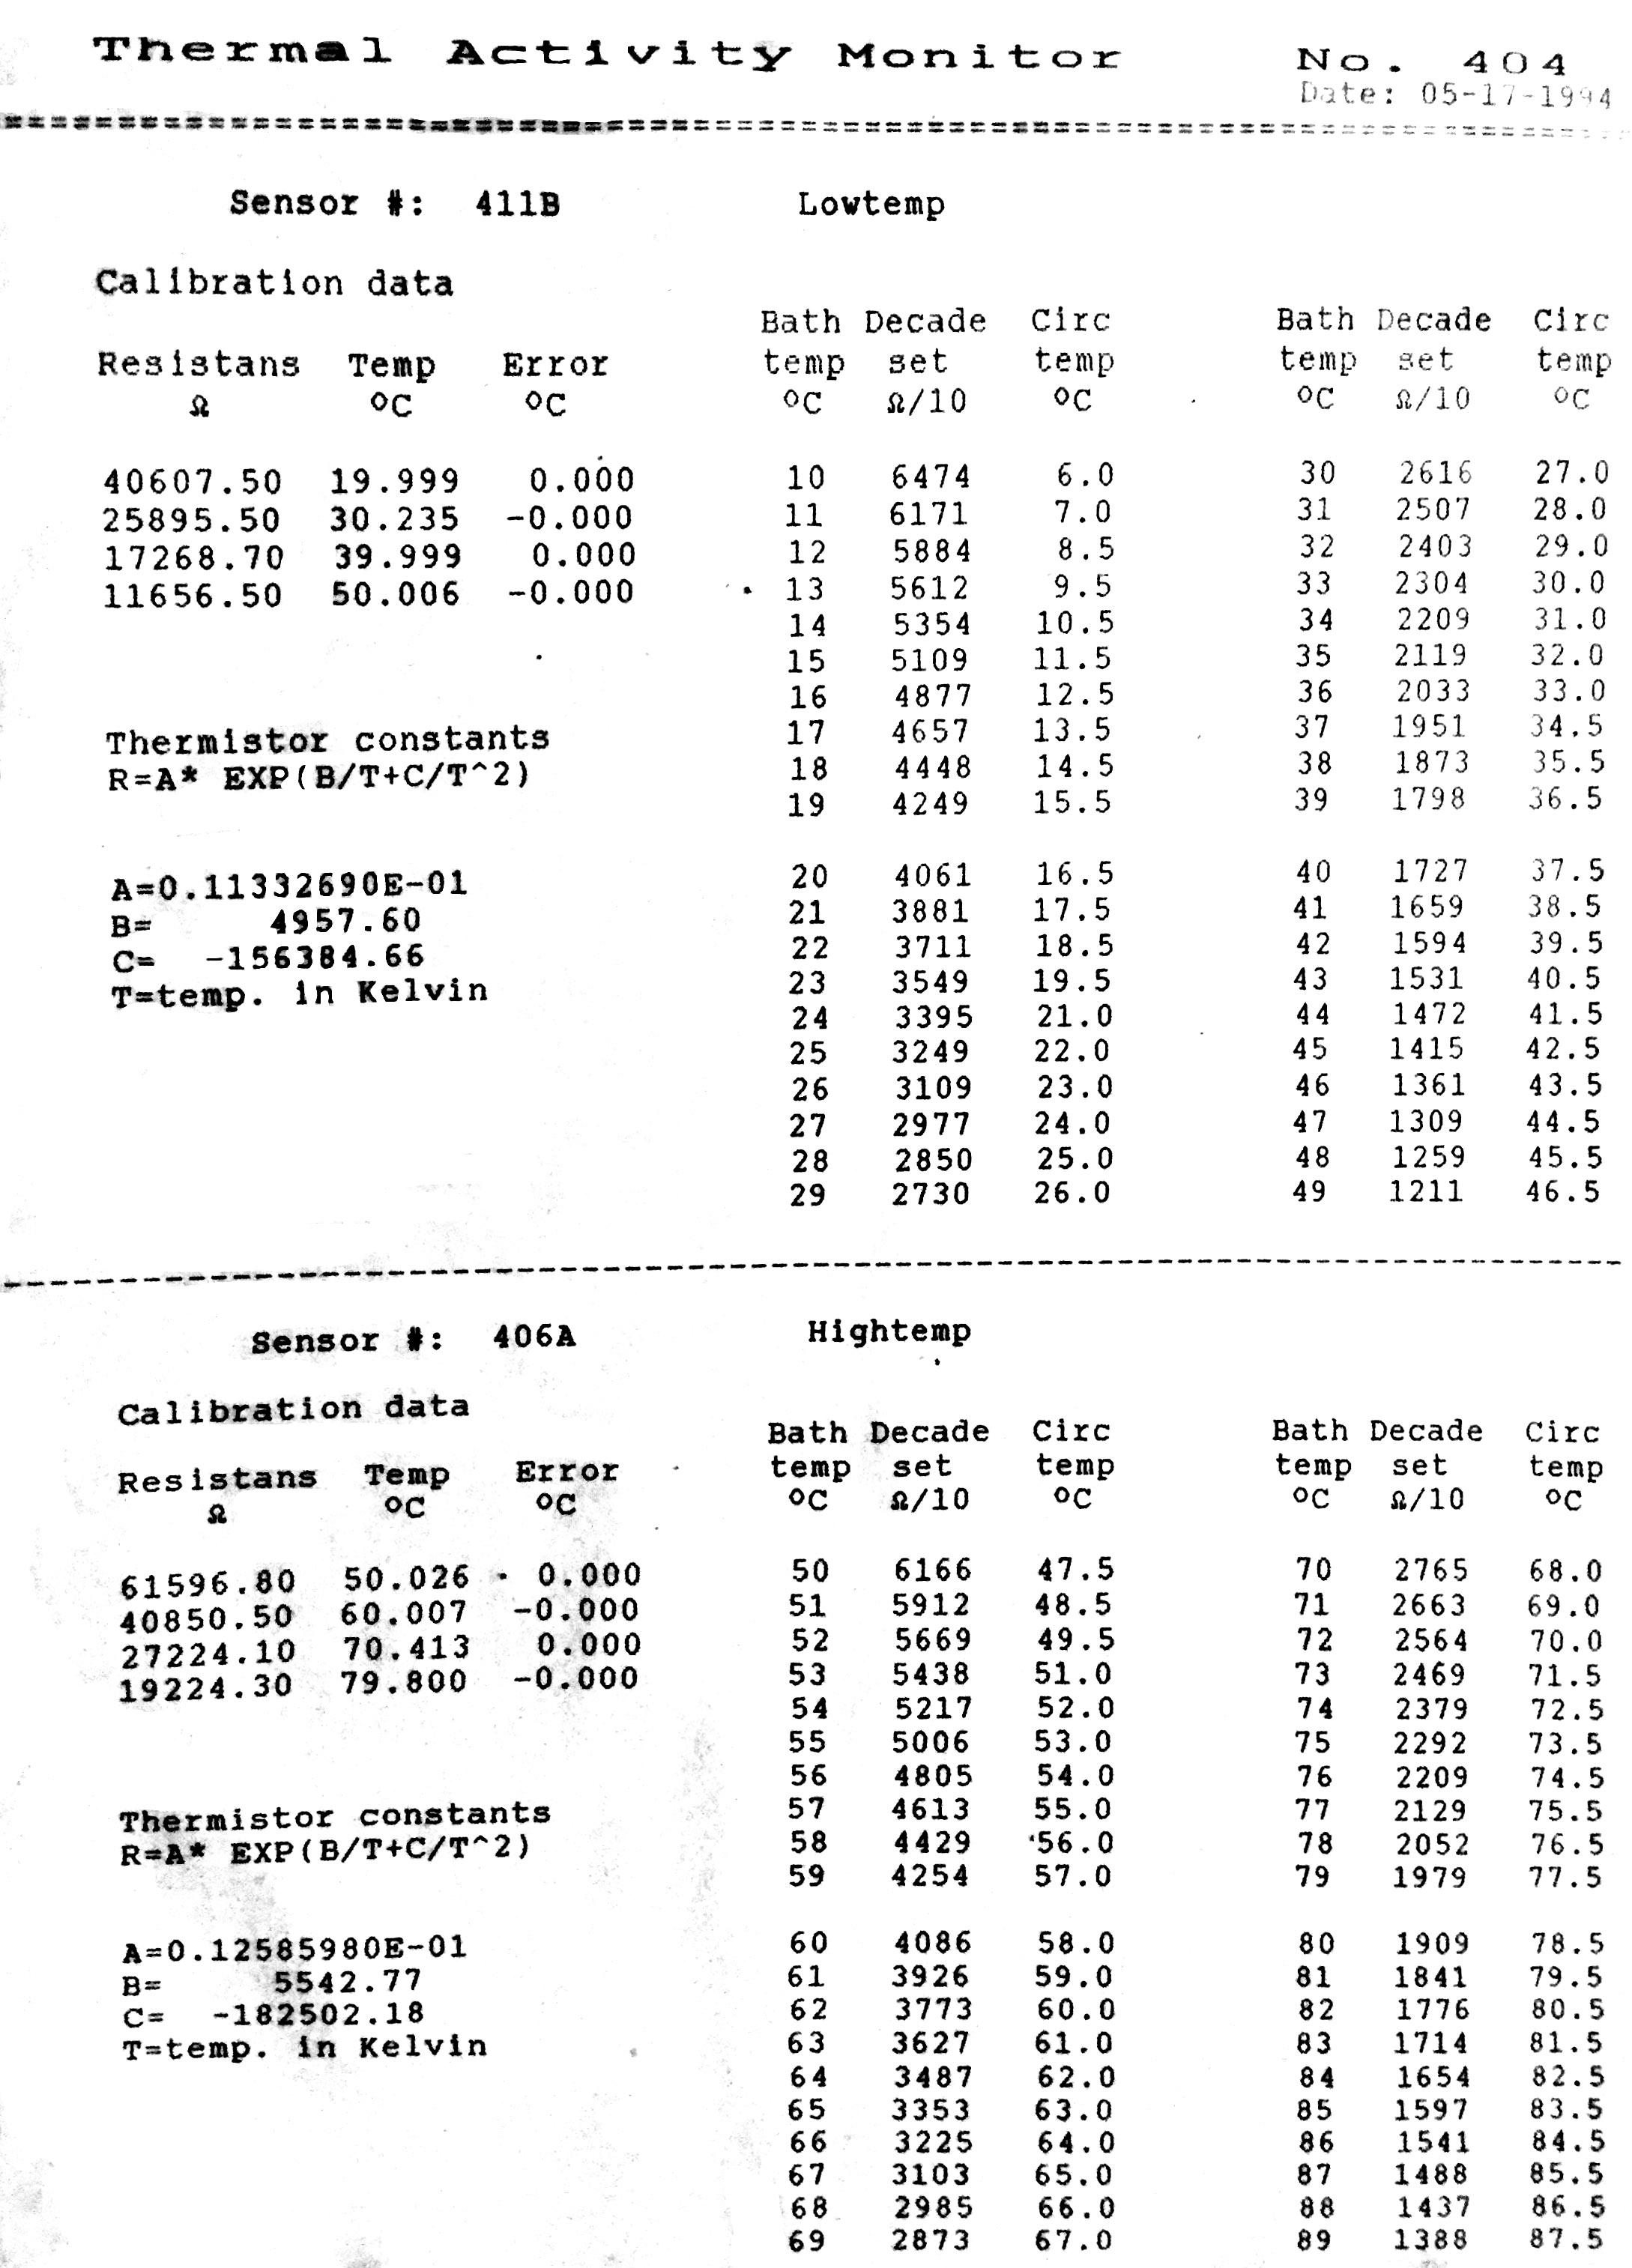
\includegraphics[height =0.95\textheight]{Figures/temperatureTable}
		\caption{Equivalencia de resistencia y temperatura en una calibraci\'on de 1994.}
		\label{fig: temperatureTable}
	\end{figure}

\chapter{Códigos}\label{anx: codigos}
	\section{Firmware microcontrolador}
		\lstinputlisting[language = C]{../MeasuringTools/micro/main.c}
		
	\section{Determinación de intervalos estacionarios en la calibración del sistema de monitoreo de temperatura}
		\lstinputlisting{../Data/TemperatureCalibration/calibration.py}
		
	\section{Software de Temperatura}\label{anx: interfaz}
		\subsection{Comunicaciones}
			\lstinputlisting{../MeasuringTools/TemperatureSoft/com.py}
			
		\subsection{Interfaz gr\'afica}
			\lstinputlisting{../MeasuringTools/TemperatureSoft/gui.py}
			
	\section{Disco 3D para sensor térmico en el calorímetro}
		\lstinputlisting{../disk_filler.scad}
			
	\section{Determinación de los valores de una calibración estática}\label{anx: staticCalibration}
		\lstinputlisting{../Data/ElectricalCalibrations/calibrations.py}